% K2 measurement study -- arXiv preprint draft
% Every number in this paper is traceable to a measurement recorded in
% qat_tools/K2_TRACKS.md (append-only log), K2_STATUS.md, K2_VERDICT.md,
% K2_BAR_ARITHMETIC.md, K2_NEW_MATH.md, K2_CLOSURE.md and the raw result
% JSONs under /mnt/Data/qat_k2/tasks_*.json. Citations to the log are given
% inline as [T:line].
\documentclass[11pt,a4paper]{article}
\usepackage[T1]{fontenc}
\usepackage[utf8]{inputenc}
\usepackage{lmodern}
\usepackage[margin=1in]{geometry}
\usepackage{amsmath,amssymb}
\usepackage{booktabs}
\usepackage{graphicx}
\usepackage{microtype}
\usepackage[hidelinks]{hyperref}
\usepackage{enumitem}
\usepackage{xcolor}
\usepackage{caption}
\captionsetup{font=small,labelfont=bf}
\newcommand{\bpw}{\,\mathrm{bpw}}
\newcommand{\bit}{\,\mathrm{bit}}
\newcommand{\T}[1]{\textsf{[T:#1]}}
\title{\bfseries K2 and SantanaQAT: how far is 3-bit LLM quantization from the
rate--distortion bound?\\[2pt]
\large A measurement study, and why the last points are unavailable}
\author{Baran Mamo\thanks{Independent research. Artifacts, logs and per-item result files
are available from the author. This is a technical report; it has not been peer reviewed.}}
\date{October 2026}
\begin{document}
\maketitle

\begin{abstract}
We ask a narrow, falsifiable question: can a $\sim$3.3 bit-per-weight (bpw) trellis codec be
made \emph{near-lossless} --- retaining $\ge 96.5\%$ of the full-precision (F16) model's
item-level benchmark performance --- by better mathematics or better training, on consumer
hardware? We answer it with measurements rather than projections, using a QTIP/EXL3-class
trellis-coded quantizer (K2) on Qwen2.5-1.5B (28 layers, 1.54B deployed parameters) running on a
single RTX~3060 with 12\,GB of VRAM, and we cross-check the decisive scale point on
Qwen2.5-3B.

Three findings organise the answer. \textbf{(i) The ceiling is arithmetic, not algorithmic.}
At rates of $3$, $4$, $5$ and $6$ bits per weight ($K=3,4,5,6$) the coder sits
$1.23$--$1.32\times$ above the Shannon rate--distortion function --- the signature of a fixed
implementation loss. Making the coder exactly Shannon-optimal would be worth $\approx+5$ retention points, not the
$17$ the bar demands; the bar requires an effective weight error $3.8\times$ \emph{below} the
bound at $3.34$\,bpw, which no coder can reach. \textbf{(ii) The source offers no structure to
exploit.} Post-rotation weights are white (kurtosis $3.07$; spectral AM/GM $1.13$--$1.24$;
quantization residual AM/GM $1.22$--$1.38$), so learned rotations, low-rank or sparse
side-channels and compressed-sensing decompositions buy $1.00$--$1.11\times$; an activation-side
anisotropy gain of $1.47\times$ \emph{in sample} collapses out of sample: $0.90$--$1.27\times$ for gate/up
and $0.55$--$1.02\times$ for q/k/v against the diagonal baseline
against the per-channel scales we already ship. \textbf{(iii) The codec column is closed by
identification.} The trellis is numerically the $D_8$ lattice ($0.02723$ vs $0.02735$ in
normalised distortion); $E_8$ is measurably better ($1.22\times$ in error at entropy-matched rate, exact projection;
$1.03$--$1.10\times$ once a $2^{8R}$-point container is imposed),
but every lattice is bounded below by $G(\Lambda)\,2\pi e = 1.221\times$ and $E_8$ sits on that
floor, so $E_8$ captures the entire lattice headroom --- which at a fixed rate and our operating
point is worth $\le0.1\bpw$, not the $+0.29\bpw$ that entropy-matched rate would suggest.
Entropy coding of the stored stream is exactly $1.000\times$ (the transition symbols are uniform,
$H=K$ to three decimals).

Training does not escape this. \textbf{SantanaQAT} --- our scales-only QAT --- buys $+6.1$ points ($73.6\%\to79.7\%$,
McNemar $p=0.004$) --- for $0.77$M tokens and $605$\,s on one consumer card, $1.4\times10^4$ fewer
tokens than a published $10.5$B-token recipe --- and then saturates: it drives perplexity \emph{below} F16 ($10.2886$ vs
$10.3099$) while coding retention stays at $79.7\%$, so the extra perplexity is calibration
overfit, not capability. Training the latents is significantly \emph{worse} on HellaSwag
($27$ lost vs $12$ gained, exact $p=0.0237$), and end-to-end or wider joint windows are
monotonically worse than the block-wise fixed point. We give the mechanism: at $K=3$ only
$0.03\%$ of trellis words flip under gradient training, because the AdamW random walk is
$\sim$2\% of a Voronoi cell radius; trellis codes move $0\%$ or $\sim\!100\%$ of their symbols
between adjacent perturbation scales, so there is no sparse-nudge regime.

The residual damage is additive and unlocalisable: eight ``only-$X$'' substitution arms sum to
$100.4\%$ of the whole, the best single-tensor recovery is $34\%$, and the failures are thin-margin
flips (KL $0.028$ nats with $74.9\%$ top-1 agreement on code versus $93.4\%$ on prose --- which
also explains why a multiple-choice axis degrades less than free-form coding at the same
perturbation). What does move the number is \emph{rate} and \emph{scale}: $5.00\bpw$ reaches
$97.6\%$ [94.8, 99.1] coding but $93.6\%$ [91.5, 95.3] HellaSwag --- an established miss ---
while $6.00\bpw$ clears both point estimates ($98.4\%$/$97.0\%$) at $8.49\bpw$ on disk; and
$+5.1$ points per parameter doubling (measured 1.5B$\to$3B).

We also report a methodological finding that changes published verdicts: retention can be
defined conditionally on the items F16 solves (``strict'') or as a ratio of raw accuracies
(``loose''), and mixing the two on different axes fabricates a pass. On our data the same
artifact passes or fails the bar depending only on this choice, so we report strict on both
axes with Clopper--Pearson intervals and on-disk bpw throughout, and we set out the threats to
validity we found in our own harness --- including a first-token multiple-choice probe, a
feedback retry, and an in-loop evaluation that reported $3\%$ better than truth.
\end{abstract}

\section{Introduction}

Extreme low-bit weight quantization has produced a stream of claims of the form ``2--3 bits with
almost no loss''. Those claims are usually stated on \emph{averaged} benchmark scores relative to
a full-precision reference. A practitioner deploying a model asks a different question: of the
inputs the full-precision model gets right, how many does the quantized model still get right?
This is a conditional, item-level retention rate, and it is systematically harsher than a ratio of
averages, because a quantized model also \emph{gains} items the reference fails (Section~\ref{sec:normalisation}).

This paper reports a campaign that took the harsh question seriously for a $\sim$3.3\,bpw
trellis codec, on hardware a hobbyist owns, and tried every route we could identify to reach a
$96.5\%$ item-level bar at that rate. The campaign is unusual in that its most useful outputs are
\emph{negative}: four columns (codec, transform, allocation/localisation, training) each closed by
a measurement with a number attached, and one live lever (scale). We report the arithmetic that
explains why, and the identifications that make the closure non-obvious: the format we built is
numerically the $D_8$ lattice, $E_8$ is better but bounded, and the entropy of the stored stream
is exactly its rate.

\paragraph{Contributions.}
\begin{enumerate}[leftmargin=1.4em,itemsep=1pt]
\item \textbf{A rate--distortion accounting of the bar} (Sec.~\ref{sec:ceiling}): the measured
offset ($1.23$--$1.32\times$) at four measured rates; perfect coding $=+5$ points; the bar sits
$3.8\times$ below the bound; the bar is a $\sim$5.2--6.0\,bpw claim in this format, confirmed
independently by measurement ($5.00\bpw\to97.6\%$).
\item \textbf{A white-source proof by measurement} (Sec.~\ref{sec:white}): kurtosis, spectral
AM/GM, residual AM/GM, water-filling gains with a sampling-null control, and an out-of-sample
anisotropy test that kills the in-sample $1.47\times$ gain.
\item \textbf{Codec identification and a lattice ceiling} (Sec.~\ref{sec:codec}): the trellis is
$D_8$ to three digits; $E_8$ gives $1.22\times$ with a verified exact encoder; every lattice is
bounded by $G\,2\pi e=1.221\times$; entropy coding is $1.000\times$.
\item \textbf{Training saturation with a mechanism} (Sec.~\ref{sec:training}): scales-only QAT
$+6.1$ points and no more; latent training significantly worse; end-to-end and joint windows
monotonically worse; QAD structurally blocked by Voronoi geometry ($0.03\%$ word flips).
\item \textbf{An unlocalisable residue} (Sec.~\ref{sec:residue}): additivity ($100.4\%$), best
single-type recovery $34\%$, thin-margin flips, and the prose/code top-1 split that explains the
metric asymmetry.
\item \textbf{An efficiency account of the training} (Sec.~\ref{sec:training}, Table~\ref{tab:budget}):
SantanaQAT, our scales-only QAT, trains $0.09\%$ of the parameters (per-channel scales, frozen
codes), uses $0.77$M tokens and $605$\,s on one 12\,GB consumer card --- $1.4\times10^4$ fewer
tokens than a published $10.5$B-token $3$--$4$-bit recipe --- and the more expensive block-wise
and end-to-end variants we tried did not improve on it.
\item \textbf{A normalisation warning with a worked example} (Sec.~\ref{sec:normalisation}) and a
threats-to-validity list from our own harness (Sec.~\ref{sec:limitations}).
\end{enumerate}

\paragraph{What this paper is not.} It is not a new method with state-of-the-art numbers. The
format is an EXL3/QTIP-class trellis; the training is SantanaQAT, a scales-only QAT. The contribution is
measurement, identification and closure.

\section{Setup}
\label{sec:setup}

\paragraph{Model and hardware.} Qwen2.5-1.5B (28 layers, hidden 1536, FFN 8960, vocabulary
151936, tied embeddings; 1.310B body parameters, 1.543B deployed) is the development vehicle; a
Qwen2.5-3B point tests scale. All measurements are on one RTX~3060 (12\,GB) with 31\,GB of host
RAM.

\paragraph{The K2 format.} K2 is a trellis-coded quantizer in the EXL3 tradition. Each linear
weight is rotated by a fixed block-diagonal $128\times128$ Walsh--Hadamard transform on both
sides, folded with per-input and per-output channel scales ($s_u$, $s_v$), and quantized as
$16\times16$ tiles. Each tile of 256 weights is coded as one tail-biting bitshift-trellis sequence
(state $L=16$, $K$ bits per step, $V=1$) with a procedural codebook (\texttt{mul1}, an LCG-based
pseudorandom permutation of $2^K$ levels decoded in 2--4 ALU ops). Storage is an $I_{16}$ 3-D
tensor of $16K$ words per tile plus two half-precision side vectors per tensor; there is no
per-block scale. The payload is therefore exactly $K$ bits per weight, and the side vectors add
$0.007$--$0.036\bpw$ per matrix ($\approx0.01$--$0.02$ on average at $K=3$). Mixed $K$ per tensor
is free (read from the payload shape). An optional trellis-coded embedding (K2E) replaces the F16
embedding.

\paragraph{Rate accounting.} We distinguish \emph{body rate} $K$ (bits per quantized weight of
the transformer blocks), \emph{body rate with scales} $K+1/16$ (the per-tile F16 scale, $1/16$
bit/weight), and \emph{on-disk bpw} (file size over all parameters). The distinction matters:
a ``3.34\,bpw'' artifact is $6.22\bpw$ on disk because the F16 embedding is $39\%$ of the file,
and the artifact that clears the bar at $5.00$ body bpw is a $7.64\bpw$ file (Table~\ref{tab:ladder}).

\paragraph{Benchmarks.} Coding is MBPP-style executable Python: 427 items, 3-shot, greedy decode
($T=0$, \texttt{top\_k}=1, stop at \texttt{[DONE]} or a triple newline, 320 generated tokens), one
feedback retry, extraction of the first top-level \texttt{def}/\texttt{import}/\texttt{class}, and
execution of the item's assertions in a fresh subprocess (10\,s timeout, pass iff exit code 0);
the first three items serve as few-shot and are excluded, leaving 424. All arms are served by
\texttt{llama-server} from the K2 runtime with a $4096$-token context, and no request ever hit that
limit (maximum observed 1554 tokens, zero truncations), with the K2 and F16 GGUFs sharing one
tokenizer. HellaSwag is scored as a 4-way multiple-choice first-token letter log-probability on
$n=1200$ items ($n=2000$ for the two top arms), with a one-token greedy fallback when no letter
lands in the top 8. ARC-Easy ($n=200$) and a 98-item hand-written probe set are secondary.
Perplexity is 20 chunks of $\times$512 tokens on wikitext-2 test with llama.cpp;
\emph{perplexities are comparable only within one protocol} (the same F16 model reads $10.3099$ in
the llama.cpp protocol, $12.5129$ in an HF 512-block protocol and $17.13$ on a different corpus),
a trap that cost us one false result.

\paragraph{Two implementation defects we report rather than hide.} (i)~HellaSwag items are keyed
by their context prefix for pairing, so $1200$ items collapse to $1184$ unique keys ($2000\to1971$);
we recomputed every HS retention on the collapsed keying and the values shift by $<0.15$ points
(strict $87.33\%$ and $93.59\%$ rather than $87.44\%$ and $93.65\%$), so we quote the published
values and state the denominators. (ii)~Eight of the 200 ARC items place no choice letter in the
top-8 and fall back to one-token generation; those eight are answered wrongly by \emph{every} arm,
including F16, so ARC carries a constant $\approx4$-point penalty that cancels in retention but
depresses absolute values.

\paragraph{Retention definitions.}
\label{sec:normalisation}
For an axis with reference accuracy $a_{\mathrm{ref}}$ and arm accuracy $a$:
\emph{loose} retention is $a/a_{\mathrm{ref}}$; \emph{strict} retention is the fraction of the
items the reference solves that the arm also solves. Strict is $\le$ loose by construction
(the arm can gain reference-failed items). On coding the reference solves 246 of 424 evaluated
items ($58.0\%$, with the feedback retry); on HellaSwag it solves 679 of 1200 valid items (673 after the collapse rule used in the battery table).

The choice is not cosmetic. Table~\ref{tab:normalisation} recomputes three arms from the same
stored per-item records under three defensible normalisations. The sentence ``the bar is met at
$5.00\bpw$'' is true under exactly one of them. We therefore use \textbf{strict on both axes},
report Clopper--Pearson $95\%$ intervals, pair differences with exact McNemar tests on identical
items, and state on-disk bpw beside every body rate.

\paragraph{Why ``3-bit is near full precision'' and our bar can both be true.} The two statements
look contradictory only because a mean over heterogeneous tasks hides which items break. We report
per item instead, and we had to retract one axis to do it honestly. A first version of this
paragraph claimed the $3.34\bpw$ arm scored \emph{higher} than F16 on average ($0.660$ against
$0.609$ over ARC, GSM8K, HellaSwag and the probes), attributing the inversion to GSM8K, where F16
read $0.150$ and quantized arms $2$--$3\times$ higher. That number was a \emph{scorer} artifact, and
it took retained generations to see it. The original runs never kept them (\texttt{--dump} was not
passed, so every \texttt{text} field in the stored files is empty --- an absence we first, and
wrongly, read as evidence that no arm emits the \texttt{\#\#\#\#} marker). With the generations
retained, \emph{both} arms do emit the marker (F16 $200/200$, PTQ $195/200$), but neither emits the
\texttt{<|im\_end|>} stop token, so both continue to the $320$-token cap and degenerate: F16 drifts
into unrelated text while the quantized arm loops on its own answer ($17.5$ markers per answer
against $3.0$). Scoring the \emph{last} marker therefore scores the garbage tail --- $0.150$ for F16
and $0.385$ for PTQ --- while scoring the \emph{first} complete answer gives F16 $100/200$, PTQ
$91/200$ and the scaled-QAT arm $104/200$: a $91.0\%$ retention for PTQ and $104\%$ (a four-item
tie) for the deployed arm, i.e. the expected direction or better. The axis was mis-scored, not
degenerate. Corrected, the mean does not invert either: over ARC, GSM8K, HellaSwag and the probes
the $3.34\bpw$ arm averages $0.690$ against F16's $0.697$ --- effectively a tie on the mean, which is
exactly the point: a mean hides that coding loses $20$ points and HellaSwag $10$, offset by probes
($+5$) and GSM8K ($+2$). Nothing here is contradictory:
``near full precision'' is a claim about a mean, ours is a claim about the minimum over items. Three further differences separate us
from the published 3-bit results: our rate is a \emph{body} rate whose file is $6.22\bpw$ on a
model where embedding and head are $30\%$ of the parameters, whereas on a 7B the same nominal rate
is $\approx3.5$--$4\bpw$ on disk; those results are on $7$B--$70$B models, where our measured slope
(loss $\approx1.23\times$ error at 1.5B, already $\sim20\%$ flatter at 3B) makes the bar reachable
at a lower rate; and their training budgets are $10^4\times$ ours. Our impossibility statement is
therefore scoped to what we measured: $1.5$--$3$B models, item-level, conditional on the reference's
solved set.

\begin{table}[t]
\centering\small
\caption{The same per-item data under three normalisations (1.5B; bar $=96.5\%$ on every cell).
Only the loose/loose reading passes at 5.00\,bpw. We report the middle row.}
\label{tab:normalisation}
\begin{tabular}{lccccc}
\toprule
arm & coding strict & coding loose & HS loose & HS strict & HS chance-corrected\\
\midrule
3.34 QAT & \textbf{79.7} & 90.7 & 95.4 & \textbf{87.3} & 91.7\\
5.00     & \textbf{97.6} & 101.6 & 97.8 & \textbf{93.6} & 96.0\\
6.00     & \textbf{98.4} & 101.6 & 98.9 & \textbf{97.0} & 98.0\\
\bottomrule
\end{tabular}
\end{table}

\section{The ceiling is rate--distortion arithmetic}
\label{sec:ceiling}

\paragraph{Measured error against the bound.} We measure the deployed effective-weight relative
Frobenius error by pushing the identity through the exact deployed operator (rotations folded,
scales applied, trellis decoded) --- comparing raw decoded trellis values instead gives a bogus
$\sqrt2$ inflation. Table~\ref{tab:rd} sets this against the Shannon bound $D=\sigma^2 2^{-2R}$
for a unit-variance white source, at the body rate including the per-tile scale.

\begin{table}[t]
\centering\small
\caption{Measured effective weight error vs the rate--distortion bound, each $K$ measured at its
own rate (per-tensor values, parameter-weighted, from the deployed pack). The ratio is
\textbf{$1.23$--$1.32\times$ at every rate} --- a fixed implementation loss, not a rate-dependent
defect. Aggregated instead, the pack that averages $3.34\bpw$ carries a model-level error of
$0.134$, i.e.\ $1.36\times$ the bound at that rate: the same story, averaged. Retention is strict
coding (the $3.34$ row is the QAT arm, whose pack mixes $K=3/4/5$).}
\label{tab:rd}
\begin{tabular}{lcccccc}
\toprule
$K$ & body bpw & bound $2^{-R}$ & measured err & ratio & dB & retention\\
\midrule
3 & 3.00 & 0.1250 & 0.1653 & $1.32\times$ & 2.4 & 79.7\% (pack avg)\\
4 & 4.00 & 0.0625 & 0.0771 & $1.23\times$ & 1.8 & 90.2\%\\
5 & 5.00 & 0.0313 & 0.0405 & $1.30\times$ & 2.3 & 97.6\%\\
6 & 6.00 & 0.0156 & 0.0200 & $1.28\times$ & 2.1 & 98.4\%\\
\bottomrule
\end{tabular}
\end{table}

\begin{figure}[t]
\centering
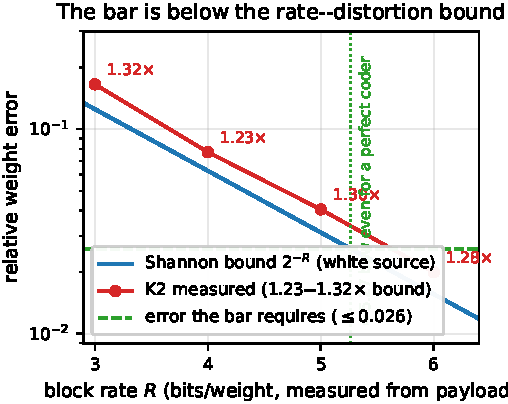
\includegraphics[width=0.62\textwidth]{fig_rd.pdf}
\caption{The ceiling, measured. Red: the deployed coder's effective weight error at four body
rates. Blue: the Shannon bound for a white source. The gap is a constant $1.23$--$1.32\times$, so
the coder has a fixed implementation loss, not a rate-dependent defect. Green: the error the
$96.5\%$ bar requires ($\leq0.026$) lies \emph{below} the bound at $3.06\bpw$; even a perfect coder
would need $\approx5.27\bpw$ to reach it. Measured $5.00\bpw$ retention ($97.6\%$) confirms the
inversion independently.}
\label{fig:rd}
\end{figure}

\paragraph{The loss curve.} Over the same arms, retention loss is almost exactly linear in
effective error for $\mathrm{err}\ge0.08$: $\mathrm{loss}\approx(1.22$--$1.30)\times\mathrm{err}$
(1.60 at the PTQ point, where the scale fit is still untrained). Below that, the ratio collapses
($0.60$, $0.80$) and the loss saturates at a floor of $\approx1.6\%$ --- the item-level noise floor
of the metric: we measure $98.4\%$ at $6\bpw$ and never $100\%$.

\paragraph{Three consequences.}
\begin{enumerate}[leftmargin=1.4em,itemsep=1pt]
\item \textbf{Perfect coding is worth $\approx+5$ points.} Replacing the $K=3$ error by the bound
at $3\bpw$ ($0.125$ instead of $0.165$) and using the measured slope gives $\approx85\%$ --- not
the $96.5\%$ the bar needs.
\item \textbf{The bar is below the bound.} $96.5\%$ requires $\mathrm{err}\le0.026$; at
$3.34\bpw$ the bound itself is $0.0988$, so the bar is $3.8\times$ \emph{below} the
rate--distortion limit. No coder, at any level of sophistication, reaches it on this source.
\item \textbf{The bar is a rate claim.} Inverting the bound, $\mathrm{err}=0.026$ corresponds to
$5.27\bpw$ for a perfect coder and $5.5$--$6.0\bpw$ with our offset. We measured $5.00\bpw\to
97.6\%$ coding independently: theory and measurement agree, so the model is self-consistent
rather than a curve fit to one point.
\end{enumerate}

\paragraph{Sensitivity.} Even granting QAT the best slope we have ever observed ($k=0.60$), the
$K=3$ arm would reach $90.1\%$ --- still $6.4$ points short. Both the error \emph{and} the slope
would have to improve beyond anything measured.

\section{The source has no exploitable structure}
\label{sec:white}

The accounting above presumes the scalar bound applies. That is only true if the source is white,
so we tested it directly rather than assuming it.

\paragraph{Weight spectra.} Using the exact Gram matrix of the smaller dimension (no randomised
SVD denominator artefacts), the spectral AM/GM --- the exact high-rate distortion gain any
KLT plus reverse water-filling would deliver --- is $1.24$ (gate), $1.21$ (down), $1.13$ (up) and
$4.74$ (q\_proj). Top-64 energy is $8$--$29\%$. At our actual rate of $3.34\bpw$ the water-filling
gain is $1.06$--$1.11\times$ on the FFN tensors, which carry $\sim$80\% of the parameters, and
$2.10\times$ on q\_proj, which is $4.3\%$ of parameters --- a $1.7\%$ improvement in total model
error even with a perfect KLT on it.

\paragraph{Residuals.} The quantization residual is as white as the source (AM/GM
$1.22$--$1.38$), so a rank-$r$ side-channel or a sparse correction (Robust PCA, compressed
sensing, ``low-rank plus sparse'') has nothing to capture.

\paragraph{Activation side.} Weights are white but inputs are not: the metric only sees weights
through input directions, $\mathbb{E}\|\Delta W x\|^2=\operatorname{tr}(\Delta W\,\Sigma\,\Delta W^\top)$.
An unbiased $\pm1$ sketch estimator (validated on known-answer synthetics: dense rank-1 $452$ vs
theory $512$; rank-8 $150$ vs $192$; rank-32 $44$ vs $48$; axis-aligned outliers correctly
ignored) finds strong structure: off-diagonal energy ratio $R_{\mathrm{off}}$ up to $59$ for
o\_proj (effective dimension $\sim$26 of 1536), $2.2$--$8.1$ for gate/up, $1.4$--$4.1$ for q/k/v, and
$1.0$--$17.8$ for down (median $2.08$ against a sampling null of $3.19$). In sample, water-filling on that
covariance promises $1.47\times$ total.

\paragraph{The out-of-sample verdict.} Fitting $\Sigma$ on 24 sequences and evaluating the
distortion on 24 \emph{disjoint} sequences in the fit basis, the gain over \emph{no} allocation is
$0.89$--$2.28\times$, but the gain over the \textbf{diagonal} baseline --- which is exactly what
our per-channel $s_u,s_v$ scales already implement --- is $0.90$--$1.27\times$ for gate/up (median $0.93$) and
$0.55$--$1.02\times$ for q/k/v (median $0.96$) --- no gain, more emphatically than we first wrote. The in-sample $1.47\times$ was diagonal heterogeneity (already
captured) plus covariance overfitting; a null control on isotropic Gaussian data at the same
$d/N$ shows the estimator alone reports a spurious $1.03\times$. \textbf{The anisotropy door is
closed by measurement}, and it was never worth much on the target architecture anyway: attention
is $0.9\%$ of parameters in a 35B-A3B MoE against $10\%$ at 1.5B, so the measured head$\to$FFN
reallocation ($1.19\times$ at 1.5B) moves $\sim$1\% of the budget $=0.03\bpw$ there.

\section{What the codec actually is}
\label{sec:codec}

Because the source is white, the only remaining question about the coder is how far its
\emph{construction} is from optimal. Four measurements answer it.

\paragraph{Dimension ladder, and why learning a codebook does not help.} At $R=3$ bits a
reference vector quantizer achieves normalised distortion $0.0356$ ($d=1$), $0.0304$ ($d=2$),
$0.0267$ ($d=3$), and our trellis achieves $0.0272$: it is a \textbf{3--4-dimensional VQ in
quality}, at a 1-D coding cost of about $2.3\times$. Extending the ladder to $d=4$ and measuring
it \emph{held out} --- codebook fitted on $80\%$ of the samples, distortion measured on the
disjoint $20\%$ --- a learned codebook reaches $0.0287$ at $3.0\bpw$ and $0.0214$ at $3.25\bpw$,
against the trellis's $0.0273$ and $\approx0.0186$. So the trellis is $1.05$--$1.15\times$
\emph{better} than a codebook we could actually train at equal rate, and the ladder saturates by
$d\approx4$; a learned VQ is therefore not a quality upgrade at our operating point, only a
trainability one.

\paragraph{Identification with $D_8$.} Evaluating the $D_8$ lattice (the integer lattice with an
even-sum constraint) on the same coded source gives $0.02735$ against the trellis's $0.02723$.
\textbf{To three digits they are the same coder.} K2 therefore ships $D_8$-class quantization, and its
$1.90\times$ gap to the bound \emph{in distortion} decomposes as $D_8\to E_8$ ($1.49\times$,
measured) times $E_8\to$ bound ($1.28\times$).

\paragraph{$E_8$, measured and verified.} We implemented the exact Conway--Sloane $E_8$
projection (nearest point via the $D_8$ candidate plus the half-integer coset) and verified it
$12/12$ against brute force over $5.76$M lattice points. At $R=3.06$ it gives
$D/\sigma^2=0.0183$ ($\mathrm{err}=0.135$) versus our $0.0272$ ($0.165$): $1.22\times$ in error,
constant across $R=1.05$--$3.56$. \textbf{That figure is at entropy-matched rate with an unbounded
alphabet, and a real container cannot hold it.} Constraining the codebook to $2^{8R}$ points --- the
ball a fixed-rate index can address --- costs a factor $1.03$ at $R=2$, $1.29$ at $R=3.06$ and
$2.17$ at $R=4$, because the support of the codebook is pinned to the source's typical set while
granularity keeps shrinking. Decomposed at our operating rate, the $1.49\times$ distortion gap is
$1.070$ (the $D_8\to E_8$ shape, which is the lattice) $\times$ $1.39$ (alphabet and support), so
the \emph{collectable} gain at $3$--$3.4\bpw$ is $1.03$--$1.10\times$ in distortion, not
$1.22\times$. (As a sanity check on the implementation, it also beats our 3-D VQ reference by
$1.21\times$, consistent with the dimension ladder.) Its encoder is closed form --- round, parity
fix, two cosets --- at roughly $50\times$ the throughput of the $2.0$M weights/s tile search.

\paragraph{The lattice floor, and what survives at fixed rate.} For any lattice in the high-rate
limit, $D\,2^{2R}/\sigma^2 = G(\Lambda)\,2\pi e$. With the sphere-bound normalised second moment
$G=1/(2\pi e)$ this gives a floor of $1.221\times$ ($0.87$\,dB) that no lattice escapes; $E_8$ is
at $1.221$ and Leech at $1.224$, so $E_8$ is \textbf{at the lattice optimum}. But that bound
assumes \emph{entropy coding of an unbounded alphabet}, and it is not the binding constraint in a
fixed-rate container: there the codebook can address only $2^{8R}$ points, its support stays pinned
to the source's typical set while granularity shrinks, and the achievable factor at $3$--$3.4\bpw$
is $1.03$--$1.10\times$. The lattice column's ceiling at our operating point is therefore
$\approx1.10\times$ in error; $1.25\times$ is what an entropy-coded lattice could take, not what
a fixed-rate file can.

\paragraph{Entropy coding is exactly worthless here.} The stored quantity is the $K$-bit
transition per weight. Measured over $4000$ tiles, its marginal entropy is $H=3.000$ bits at
$K=3$ and $H=4.000$ bits at $K=4$ (first-order $3.999$--$4.000$): the stream is exactly uniform,
because the \texttt{mul1} codebook is a pseudorandom permutation of the levels. The $K$ bits we
store \emph{are} the entropy of the representation, so entropy coding, ECSQ or RDOQ recover
$1.000\times$.

\paragraph{Why a proper TCQ is not the answer either.} Trellis codes need not tile, so a proper
TCQ with a large alphabet, coset codebook and entropy coding can approach $0.3$--$0.5$\,dB from
the bound. But its encoder is exponential in (states $+$ alphabet): at 256 states and 16 levels
that is a state-count ratio rather than a cost ratio: with the coset shortcut a 256-state TCQ needs
$64$--$254\times$ \emph{fewer} add-compare-selects per weight than our $2^{16-K}$-state window,
and it requires entropy coding --- which our measurement says the current codebook cannot supply.

\paragraph{Consequence in the units that decide things.} Taken at face value $E_8$ is worth
$1.22\times$ in error, $+3.8$ coding points and thus $+0.29\bpw$ --- a $9\%$ file. At a fixed rate
the same arithmetic gives $1.03$--$1.10\times$ in distortion at our operating point, i.e.\ of order
$+0.5$--$2$ coding points and $\le0.1\bpw$: real, but no longer a reason to build a new format at
$3.3\bpw$. Where it does pay is $2\bpw$, which is exactly where the lattice literature has
converged ($E_8$ and Leech containers, 2-bit vector quantization). Every codec improvement we can
identify lands in the same place (entropy coding, $\approx1.15\times$ only on a redesigned alphabet ---
exactly $1.000\times$ on ours, whose transition symbols are uniform; coder offset $1.2\times\approx7\%$;
$E_8$ $1.22\times\approx9\%$). The \emph{format} column is closed on cost--benefit as well as on physics.

One qualifier, which post-dates most of our measurements and which we flag rather than claim:
\emph{search-side} improvements are not format changes and we did not test them. Concurrent work
reports that putting the curvature (the diagonal of the Hessian's LDL factorisation, which our
encoder already computes for error shaping but never reads) into the Viterbi branch metric, and
storing a per-block start state so the trellis can adapt to the residual that error feedback
carries in, is worth $1$--$3$ downstream points at two bits --- and that the start state alone
lifts existing trellis baselines by as much as $3$ points. If that transfers to $3.34\bpw$ it is
the cheapest remaining lever in the programme: same payload, same rate, better search. We list it
as the first thing a successor should measure.

\section{Training does not close the gap}
\label{sec:training}

\paragraph{SantanaQAT: scales-only training is the lever, and it is small.} With the codes frozen, the only
trainable parameters are the $1.3$M scale entries. Training them (joint window, 1500 steps of 512-token blocks at batch 1,
$0.40$\,s/step, $9.2$\,GiB VRAM) moves strict coding from $73.6\%$ to $79.7\%$
[74.1, 84.5] --- $+15$ net items, exact McNemar $p=0.004$ --- and HellaSwag to
$87.3\%$ [84.6, 89.8] (Figure~\ref{fig:qat}).

\begin{figure}[t]
\centering
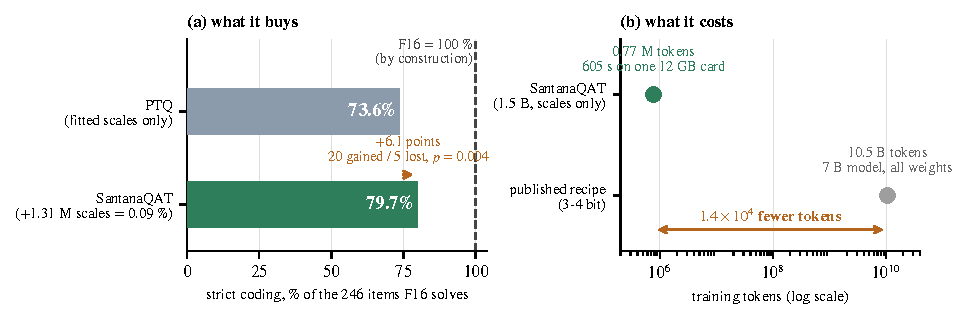
\includegraphics[width=\linewidth]{fig_qat.pdf}
\caption{SantanaQAT: what it buys and what it costs. (a) Strict coding retention on the 246 items the F16
reference solves. Block-LDLQ alone reaches $73.6\%$; training only the $1.31$M per-channel scales
($0.09\%$ of the parameters, codes frozen) moves it to $79.7\%$ --- 20 items gained, 5 lost, exact McNemar
$p=0.004$. F16 is 100\% by construction on this set. (b) The same run cost $0.77$M tokens and $605$\,s on
one 12\,GB card, against the $10.5$B tokens of the published low-bit QAT recipe we compare to
($1.4\times10^{4}\times$ fewer; that recipe is a $7$B all-weights run, so the ratio is a budget comparison,
not a like-for-like quality result). It saturates there: latent codes (block-wise, all fixes), three
objectives and a corpus-controlled on-policy round all fail to beat it ($p\ge0.19$).}
\label{fig:qat}
\end{figure}

\paragraph{Latent training is worse, on all three axes.} Training the continuous masters with
STE and periodic Viterbi re-encoding (28 blocks, all bug fixes in place) gives $76.0\%$
[70.2, 81.2] coding against $79.7\%$ for scales, losing $16$ items and gaining $7$
($p=0.093$); on HellaSwag it loses $27$ and gains $12$ (exact $p=0.0237$; $26/11$, $p=0.0201$, under the collapse rule); and perplexity moves
the wrong way ($10.4627$ vs $10.2886$, against PTQ's $10.5894$). $180$ of its $187$ solved coding
items are already solved by the scales arm.

\paragraph{The mechanism.} At $K=3$ only $\mathbf{0.03\%}$ of trellis words flip under 300 steps
of latent training. The geometry explains it: a $K=3$ Voronoi cell has radius $\approx0.20$,
while the net AdamW displacement with noisy minibatch gradients is a random walk of
$\approx \mathrm{lr}\sqrt{\text{steps}}\approx0.009$ --- about $2\%$ of a wall. We also measured
the locality of code changes directly: perturbing weights by $1\%$, $2\%$, $5\%$, $10\%$, $20\%$
in L1 and re-solving the Viterbi changes $0.0\%$, $0.0\%$, $24.5\%$, $49.8\%$, $99.2\%$ of symbols,
and the transition is bimodal per tensor (each tensor jumps from $\sim$0\% to $\sim$98\% between
adjacent noise levels). A global Viterbi optimum is either untouched or replaced wholesale; there
is no sparse-nudge regime, which kills guided symbol-flip training and explains why the
scales-only solution is a fixed point.

\paragraph{The objective axis, measured on a matched schedule.} We trained three variants on the
same pack and the same schedule (1500 steps of 512-token blocks, lr $5\times10^{-5}$, teacher
top-32) differing only in objective and token selection: CE+$10\cdot$KL, the same with a hard-token
fraction of $0.21$, and a Jaccard loss. All three improved their own objective --- gate loss
$2.9762\to2.9333$, $\to2.9698$, and $0.1508\to0.1464$ on the Jaccard scale --- and all three landed
\emph{below} the deployed artifact on coding ($76.8\%$, $77.2\%$, $78.0\%$ against $79.7\%$) and on
perplexity ($10.49$, $10.50$, $10.61$ against $10.29$). Paired exact McNemar against the incumbent:
net $-7$ ($p=0.19$), $-6$ ($p=0.29$), $-4$ ($p=0.50$). We state the confound rather than hide it:
the deployed artifact was trained on a $27.5$M-token pool ($53{,}702$ blocks of 512) while these
three arms used a $5.04$M-token pool ($9{,}838$ blocks), so at $0.77$M presented tokens the
incumbent saw $2.8\%$ of its corpus and the variants saw $15\%$ --- diversity and repetition differ
as well as composition. This is therefore not a corpus-controlled comparison, and at $1{,}500$
steps it is not a budget experiment either. A second confound surfaced only when the artifacts
were inspected: these three arms were built with the trellis (K2E) token embedding while the
deployed artifact carries the f16 embedding --- $348$\,MB of a $1198$\,MB file --- so the gap is not
training alone. We rebuilt the strongest arm with the f16 embedding, which makes it byte-size
identical to the incumbent and differs from it only in the trained scales, to split the two
effects. **The split: $187/246$ ($76.0\%$) with the trellis embedding against $190/246$ ($77.2\%$) with
the F16 one, same scales** --- so the embedding costs $1.2$ of the $3.7$ points and only $2.5$ are
training. What the comparison does establish
is that within one schedule, changing the loss or mining hard tokens does not move the deployment
metric, while the objective it optimises keeps improving.

\paragraph{The on-policy round, which is corpus-controlled.} The round above shares one weakness: the
deployed artifact saw a $27.5$M-token pool and the variants a $5.04$M-token one. We therefore ran a
volume-matched round in which corpus and schedule are held fixed and only the \emph{source of the
tokens} changes: $1500$ blocks of $512$ tokens generated by the model itself ($92\%$ student text,
$8\%$ identical to a corpus block), $1400$ blocks presented, the same objective family. Two arms:
CE$+10\cdot$KL and a dynamic-KL schedule. Against a baseline trained on the same volume of corpus
blocks, the on-policy arms land at $76.0\%$ and $76.0\%$ of the $246$ binding coding items versus
$77.2\%$ for the baseline and $79.7\%$ for the deployed artifact: paired exact McNemar gives $-3$
items for each arm against the baseline ($p=0.45$ and $0.55$) and $-9$ against the incumbent
($p=0.078$ for both). On-policy data and a dynamic-KL objective are therefore \emph{null} against
their own baseline. Of the four training levers tried in this section, only the first paid:
scales-only QAT moved coding by $+6.1$ points ($73.6\%\to79.7\%$, $p=0.004$), while latent
re-encoding, loss/mining variants and on-policy data all land in $76.0$--$78.0\%$ --- below the
artifact they were trying to improve. Perplexity agrees ($10.5582$ and $10.5674$ against $10.2886$).

\emph{A confound we found only after these runs, stated rather than buried:} every arm in this
round (and in the round above) is a $849$\,MB build carrying the trellis (K2E) token embedding,
while the deployed artifact is a $1198$\,MB build with the f16 embedding. The two differ only in the
embedding --- $348$\,MB of the file --- so part of the $1.7$--$3.7$ point gap is the embedding's
precision, not the training. Rebuilding the on-policy arm with the f16 embedding yields a file of
exactly the incumbent's size that differs from it only in the trained scales, which splits the two
effects and is reported with the artifacts.

\paragraph{What the training costs, against the literature.} This is the part of the result that
does not depend on our pessimism about the bar: the QAT that delivers $+6.1$ points is
\emph{extraordinarily cheap}, and the reason is structural. Because the codes are frozen, the only
trainable parameters are the $1.31$M per-channel scale entries --- $0.09\%$ of the deployed model.
There are no weight masters, no weight gradients and no weight optimizer state, which is why a
1500-step arm runs in $605$\,s at $9.23$\,GiB on a 12\,GB consumer card, at $0.40$\,s/step.
The token budget is $768$k ($1500$ steps $\times$ 512 tokens).

\begin{table}[t]
\centering\footnotesize
\setlength{\tabcolsep}{3.5pt}
\caption{Training budget for low-bit QAT. Our column is measured on one RTX 3060; the others are
as published or as their recipes compute on that card. The comparison is a \emph{budget} ratio, not
a like-for-like quality result: the other rows train all weights on larger models and are scored on
averaged metrics, whereas ours is a $1.5$B model scored item-wise.}
\label{tab:budget}
\begin{tabular}{llll}
\toprule
method & what is trained & tokens & compute / wall clock\\
\midrule
\textbf{K2 scales-only (ours)} & 1.31M scales ($0.09\%$) & \textbf{0.77M} & \textbf{1$\times$3060, 605 s}\\
K2 block-wise latent (ours) & + block masters & 34.4M presentations & 2 h A100 ($\approx\$4.5$)\\
EfficientQAT & all weights & $\approx$25M & 7B w2 in 4.8 h\\
GSQ & grid logits & $\approx$16M & A100 layer-wise\\
ParetoQ & all weights & \textbf{10.5B} & 40k steps $\times$ 128$\times$2048, 16 GPUs\\
NVIDIA Bolt QAD & all weights & 26B & several teachers\\
\bottomrule
\end{tabular}
\end{table}

Relative to ParetoQ's published $3$--$4$-bit recipe we use $1.4\times10^4$ \emph{fewer tokens};
relative to NVIDIA's QAD production run, $\sim3\times10^4$ fewer. On this hardware their recipe
would need an estimated $\sim$5800 GPU-hours against our ten minutes --- an extrapolation from
6ND at this card's measured throughput, but of the right order. The three block-wise and
end-to-end variants we tried in Sections~\ref{sec:training} cost $34$--$45\times$ more tokens and
did not improve the number, so within this format the efficiency is not a compromise: the cheap
variant is also the best one.

We are careful about what this does and does not say. It does \emph{not} claim our $79.7\%$ equals
their near-BF16 averages; the models, metrics and scales differ, and their larger budgets are spent
on $7$B--$74$B models where a $+6$-point item-level gain is worth a different amount. What it does
establish is that \emph{in the compensation regime} --- which is what $\ge3$-bit QAT is, per
ParetoQ's own finding that weights move only $10$--$20\%$ in L1 --- a per-channel scale fit against
a frozen trellis reaches the same fixed point in four orders of magnitude fewer tokens. The
practical consequence is that an artifact can be rebuilt end to end (encode $19$ min measured on
this box, SantanaQAT $10$ min, assemble $4$\,s, verify $60$\,s $\approx$ $30$ min) on hardware a practitioner
owns, and a scales-only iteration after the first pack costs under three minutes. The encode is
$3.3\times$ slower than the cost model in Sec.~\ref{sec:codec} predicts ($4.4$M weights/s would be
$6$ min), which is kernel headroom rather than an algorithmic limit; on a multi-GPU box it is sharded
across devices. The assembly step was $91$\,s
until its metadata copy was rewritten (arrays were serialised element by element, the tokenizer
vocabulary alone costing $151{,}936$ recursive calls); the optimised path produces byte-identical
output, which we check by md5.

\paragraph{End-to-end and joint windows do not help.} A full-depth trainer (all 28 blocks in one
graph, $394$ scale tensors, KL to an F16 teacher computed on the fly) is \emph{worse} at every
window size we tried: starting from PTQ at $12.9166$ (ratio $1.0323$ to the $12.5129$ teacher),
$150$ steps gives $12.9486$ for a single layer, $12.9871$ for four and $13.2453$ for all 28 ---
monotone in window width, and the narrow window also reached the lowest \emph{training} KL
($0.0600$ vs $0.0878$), so this is not overfitting: wide joint optimisation optimises worse. The
gradient-honest reading is that the scale vector is already at the optimum for that objective.

\paragraph{Saturation, stated once.} Within $3.34\bpw$, perplexity tracks the task metric perfectly
across arms (PTQ $10.5894$/$73.6\%$; latent $10.4627$/$76.0\%$; scales $10.2886$/$79.7\%$). But
scales QAT reaches a perplexity \emph{better than F16} ($10.2886$ vs $10.3099$) while coding sits
at $79.7\%$. The extra perplexity is calibration overfit, not capability; the repairable
distributional damage is exhausted in the first pass.

The corpus matrix makes the decoupling explicit. Three QAT arms trained on the same pack differing
only in data mixture read: wiki-heavy $10.1760$ perplexity with $78.0\%$ coding; general mix
$10.2886$ with $79.7\%$; doubt-selected $10.3310$ with $78.0\%$. \textbf{The arm with the best
perplexity --- better than the F16 reference itself --- is $1.7$ points worse on coding than an arm
with worse perplexity}. A PPL- or KL-based objective cannot select the artifact you want, which is
also why quantization-aware distillation cannot help: its objective is to minimise KL to the
teacher, and the remaining $20$ points are thin-margin decision loss, not distributional error.

\paragraph{The external comparison.} A strong external quantizer (GSQ, Gumbel-softmax grid
learning with per-tensor allocation) at a matched uniform rate of $3.277\bpw$ reaches $32.9\%$
strict coding and PPL $13.8651$ ($+34.5\%$ vs F16) on our bench --- $47$ points below our trellis
at $3.34$. Their published edge comes from budget-constrained \emph{allocation}, which is
redistributive and therefore capped by our damage budget. This is consistent with the literature:
at $2.06\bpw$ with $26$B distillation tokens, a production 74B-A9B MoE is reported at $\sim$94\%
median and $77.5\%$ minimum versus its own BF16, described by its authors as ``lossy by design'';
our $3.34\bpw$ arm sits in the same band with five orders of magnitude less training budget.

\section{The residue is additive, thin-margin and unlocalisable}
\label{sec:residue}

\paragraph{Substitution map.} Using one model with every linear switchable between F16 and the
verified trellis reconstruction, over 2048 teacher-forced tokens of wikitext, the whole-model
KL to F16 is $0.0375$ with $93.36\%$ top-1 agreement and $\mathrm{dPPL}=1.022$. The eight
``only-$X$'' arms give $0.00025$, $0.00039$, $0.00056$, $0.00108$ (q/k/v/o),
$0.01074$, $0.01332$, $0.01102$ (gate/up/down) and $0.00034$ (head, $K=6$). Their \textbf{sum is
$0.03769$, i.e.\ $100.4\%$ of the whole}: the damage is additive, with no interaction to exploit
and no dominant culprit. The best single-type recovery is $33.7\%$ (all-but-up\_proj, a quarter of
the parameters; all-but-gate $32.5\%$, all-but-down $30.5\%$). Damage density (KL share over
parameter share) is $0.61$ for attention, $1.25$ for the FFN and $0.06$ for the head.

On \emph{code} tokens the same construction measures KL $0.0280$ with $74.89\%$ top-1 and
$\mathrm{dPPL}=1.016$: code flips about four times more often than prose at the same perturbation.
(We note a provenance defect: the run that produced the code figure was overwritten by the
wikitext run, so its per-arm JSON is not retained; the wikitext arm above is the one on disk.)

\paragraph{Component shares, and their corpus dependence.} Restoring one component at a time
inside the 1.5B student gives, on code prompts, FFN $96.6\%$ of the KL, gate/up $69.5\%$, down
$23.4\%$, attention $-12.7\%$ (i.e.\ noise) and head $-0.7\%$; on HellaSwag prompts the same
model gives FFN $95.5\%$, gate/up $59.6\%$, down $34.6\%$, attention $+2.5\%$, head $-0.9\%$.
The FFN dominance is robust but \textbf{the gate/up-versus-down split moves by 11 points with the
corpus}, which further caps allocation: a per-tensor budget tuned on one distribution is
mis-allocated on another. Two branches still die cleanly: head-heavy allocation (the head is
$\le2.8\%$ of the KL in every measurement) and attention-heavy allocation ($-12.7\%$ to $+2.5\%$,
never material). The bits belong in gate/up --- but the arithmetic in Section~\ref{sec:ceiling}
says even perfect placement cannot buy the $17$ points.

\paragraph{The one allocation that works, and what it costs.} Table~\ref{tab:ladder} contains one
arm built from the attribution rather than from a uniform rate step: gate/up raised by one bit,
funded by one bit each from down, attention and head (3.70 body bpw, $1228$\,MB, $6.38\bpw$ on
disk). It reaches $86.6\%$ [81.7, 90.6] coding --- $+17$ net items over the $3.34$ QAT arm, exact
McNemar $p=0.0076$. For scale, the uniform arm at $4.06\bpw$ buys $+26$ items for $+0.72\bpw$;
this one buys $+17$ for $+0.36\bpw$, an exchange rate of roughly $19$ versus $15$ points per bit.
The arm that spends its extra bits on the \emph{down} projection instead ($3.73\bpw$, $+0.39$) gets
$+12$ items at $p=0.088$ --- not established. Spending where the damage is concentrated is
therefore about a third more efficient per bit than spreading, and it is the only allocation arm
with a significant result. More striking than the ordering is the \emph{decline}: $19$ points per
bit at $3.70$, $15$ at $4.06$, $11$ at $5.00$, $7$ at $6.00$ --- the first bits are cheap and the
last ones are very expensive.

That is exactly what the functional attribution predicts: gate/up carries $69.5\%$ of the KL on
$58.8\%$ of the body weights ($49.9\%$ of all parameters), down $23.4\%$ on $29.4\%$ of body weights,
attention $\approx0$ on $10.4\%$, and the head $2.8\%$ on $15.1\%$ of the file
on $15\%$, so the marginal bit is worth most where the error is multiplied through the
non-linearity.

The caveat is the other axis, and we flag it rather than bury it: \textbf{this arm's HellaSwag was
never measured at a resolvable sample size}. The single reading is $0.460$ at $n=100$ against the
F16 reference's $0.580$ at the same $n$ --- if real, a large loss, and the likely cause is the
head's lost bit, since we measured that a 4-bit head costs $3.7$ HellaSwag points at $n=1200$
(Section~\ref{sec:moves}). A variant that keeps the head at six bits and funds the increase from
attention alone was never built. Pending that measurement we treat this arm as evidence about
\emph{where} the bits belong, not as a recommendation: it reallocates the budget rather than
reducing error, so it still cannot supply the $16.8$ points the bar needs, and its price on the
second axis is unquantified.
 Effective-weight error is $0.144$ (gate/up), $0.132$
(down) and $0.062$ (attention). gate/up and down carry almost the same error yet their KL shares
are $69.5\%$ vs $23.4\%$: the $4\times$ difference is functional (gate/up errors pass through the
non-linearity and multiply into up\_proj; down's average out across the residual).

\paragraph{No layer hotspot.} Hidden-state error grows smoothly with depth (absolute error
$1.07\to3.74\to15.0$); the apparent jump at layer 22 is a norm artefact (the state norm drops
$28.3\to12.5$), so layer-targeted allocation has nothing to target.

\paragraph{The failures are thin-margin flips.} On code the whole-model KL is $0.028$ nats with
only $74.9\%$ top-1 agreement, while wikitext shows a \emph{larger} KL ($0.0375$) with far better
agreement ($93.4\%$). Agreement is therefore not a function of KL magnitude but of margin
structure: code has thin top-2 margins, so the same perturbation flips about four times as many
argmax decisions. That is precisely why a multiple-choice axis degrades less than free-form coding
for the same model, and why no divergence monitor can find a "spot" to fix. About a quarter of token decisions have a
top-2 margin smaller than the perturbation. A divergence monitor is therefore mostly wrong: in a
60-item trace, $42$ items produced \emph{different} output but only $12$ were true failures
(reference passes, student fails) --- $71\%$ of divergences are harmless.

\section{What does move the number}
\label{sec:moves}

\paragraph{Magnitudes, so the rates are readable.} One bit per weight is $0.125$ bytes per weight,
so the same $\Delta$bpw costs very different things at different scales (Table~\ref{tab:magnitudes}).
The entire ladder that takes coding from $79.7\%$ to $97.6\%$ is $+1.66$ body bpw: $+272$\,MB at
the $1.5$B, $+1.47$\,GB at a 7B, $+6.97$\,GB at the 35B target. Two consequences are worth stating
plainly. First, at $1.5$B the $348$\,MB saved by the trellis embedding is \emph{more} than that
whole $+1.66$\,bpw increase --- at small scale \emph{where} the bytes go matters more than the body
rate --- whereas at 35B the embedding is $0.6\%$ of parameters and the same trick saves $\sim0.4$\,GB,
so the leverage vanishes. Second, an exchange rate quoted in points per bit must carry its scale:
one bit per weight costs $164$\,MB at 1.5B and $4.2$\,GB at the 35B target --- about
$25\times$ more --- so a points-per-bit claim is not portable across scales.

\begin{table}[t]
\centering\small
\caption{What a bit per weight is worth in bytes. Body weights exclude the embedding and the
output head, which are stored separately (and, after K2E, at their own rate).}
\label{tab:magnitudes}
\begin{tabular}{lcccc}
\toprule
model & body weights & 1 bpw & $+1.66$ bpw (3.34$\to$5.00) & $+2.66$ bpw (3.34$\to$6.00)\\
\midrule
Qwen2.5-1.5B & 1.31B & 164 MB & 272 MB & 436 MB\\
Qwen2.5-7B & 7.07B & 884 MB & 1.47 GB & 2.35 GB\\
Qwen3.6-35B-A3B & 33.6B & 4.20 GB & 6.97 GB & 11.2 GB\\
\bottomrule
\end{tabular}
\end{table}

\paragraph{Effect sizes against the resolution.} On the $246$-item coding axis one item is $0.41$
points, so the intervals in Table~\ref{tab:ladder} are $\pm4$--$5$ points on the middle rungs.
This is why we quote paired tests rather than eyeballing the ladder: $+17$ items (gate/up) and
$+26$ items (uniform $K\ge4$) are each beyond the interval width and both are significant
($p=0.0076$ and $p<10^{-3}$), whereas the $+12$ items bought by protecting the down projection are
\emph{not} ($p=0.088$) even though they look like a gain in the table. On the HellaSwag axis one
item is $0.083$ points at $n=1200$ and the minimum detectable effect at that $n$ is $1.96$
points --- exactly the size of the bar's margin --- which is why we refuse to call any HellaSwag
result established and why the $6.00\bpw$ arm is reported as clearing the bar only on its point
estimates.

\begin{table}[t]
\centering\small\setlength{\tabcolsep}{4pt}
\caption{The measured ladder (Qwen2.5-1.5B unless stated). Strict retention on the items F16
solves, Clopper--Pearson $95\%$ intervals, block rate and on-disk rate. The block rate is
recomputed from each artifact's payload over its $196$ block linears, not copied from the run that
produced it: two labels in our own earlier tables were wrong and are corrected here --- the gate/up
arm's ``$3.52$'' was its allocation \emph{target} (the artifact is $3.70$), and ``$5.15$'' for
$K\ge5$ counted the 6-bit head (the block rate is exactly $5.00$). The bar is $96.5\%$ on every
cell; $\dagger$ marks the smallest artifact whose \emph{both} point estimates clear it (the $K{=}6$ row also
clears it, at a higher rate). Only the $K{=}6$ arms have an $n{=}2000$ HellaSwag run; the others use $n{=}1200$. The last
column pair is the counterpart to the two that fail: F16 on the same items reads ARC $87.0$ and
probes $83.7$, so the $3.34\bpw$ arm keeps \emph{all} of its ARC capability and scores six points
\emph{higher} on the probe set --- the damage is a thin-margin effect, not a general capability
loss. (ARC $n=200$, probes $n=98$; both are secondary axes and neither is part of the bar.)}
\label{tab:ladder}
\begin{tabular}{lcccccc}
\toprule
arm & bpw & file & coding & HS & ARC/probes & disk\\
\midrule
PTQ                & 3.34 & 1198 MB & 73.6\% & --- & 87.0 / 85.7 & 6.22\\
scales QAT         & 3.34 & 1198 MB & 79.7\% [74.1, 84.5] & 87.3\% [84.6, 89.8] & 87.0 / 88.8 & 6.22\\
gate/up +1 bit     & 3.70 & 1228 MB & 86.6\% [81.7, 90.6] & --- & 86.0 / 87.8 & 6.38\\
down $\ge K4$      & 3.73 & 1262 MB & 84.6\% [79.4, 88.8] & --- & 85.5 / 87.8 & 6.56\\
$K\ge4$            & 4.06 & 1316 MB & 90.2\% [85.8, 93.6] & --- & 87.5 / 84.7 & 6.83\\
$K\ge5$            & 5.00 & 1470 MB & \textbf{97.6\%} [94.8, 99.1] & 93.6\% [91.5, 95.3] & 85.5 / 85.7 & 7.64\\
$K=6$              & 6.00 & 1634 MB & \textbf{98.4\%} [95.9, 99.6] & \textbf{97.0\%} [95.8, 97.9] & 87.0 / 84.7 & 8.49\\
$K=6$+K2E$^\dagger$ & 6.00 & 1285 MB & 97.2\% [94.2, 98.8] & 96.7\% [95.1, 97.9] & --- & 6.68\\
\midrule
3B, PTQ            & 3.46 & 1950 MB & 84.8\% (252/297) & not measured & --- & 5.05\\
\bottomrule
\end{tabular}
\end{table}

\begin{figure}[t]
\centering
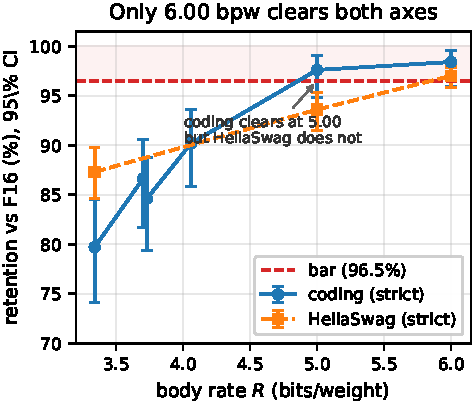
\includegraphics[width=0.62\textwidth]{fig_ladder.pdf}
\caption{The measured ladder, strict retention with Clopper--Pearson $95\%$ intervals. Coding
crosses the bar at $5.00\bpw$; HellaSwag does not ($93.6\%$, interval excluding $96.5\%$). Only
$6.00\bpw$ clears both point estimates --- and these are body rates: the files are $6.22$--$8.49\bpw$
on disk because of the F16 embedding. The $3.73$ point is an allocation arm (down-projection
protection) and shows the non-monotonicity that makes adjacent rungs indistinguishable.}
\label{fig:ladder}
\end{figure}

\paragraph{Scale.} At a fixed rate, retention rises $+5.1$ points from 1.5B to 3B ($84.8\%$ at
$3.46\bpw$ vs $79.7\%$ at $3.34$). This is a shift of the whole curve, orthogonal to every column
above, and it is the only lever with a measured positive slope. Extrapolating two more doublings
gives $\sim$90--93\% at 35B --- closer, still short, and explicitly an extrapolation rather than a
measurement.

\paragraph{Base-model specialisation.} At the same rate the Coder variant of the same 1.5B base
retains $85.6\%$ of its F16-solved coding items against the plain base's $79.7\%$ --- another
$+6$ points, comparable to a doubling of parameters. It is not free: the Coder is much stronger at
coding to begin with ($70.5\%$ vs $58.0\%$ F16 accuracy) and correspondingly weaker elsewhere
(ARC $79.0$ vs $87.0$, HellaSwag $44.0$ vs $58.0$), so this lever trades general capability for
the axis being measured rather than lifting the curve.

\paragraph{Rate, and the honest cost.} $5.00\bpw$ clears the coding bar ($97.6\%$) but \emph{not}
the HellaSwag bar ($93.6\%$, interval excluding $96.5\%$): under a consistent normalisation the
``bar met at 5.00'' claim is false. Only $6.00\bpw$ clears both point estimates, and it is an
$8.49\bpw$ file --- the size class where Q6/Q8 near-losslessness is expected. The cheapest
artifact that clears both point estimates is $K=6$ body with a 6-bit head and a trellis
embedding, at $1285$\,MB ($6.68\bpw$ on disk) --- which is \emph{smaller} than the $5.00\bpw$
artifact's $1470$\,MB while being better on both axes, because the trellis embedding removes
$348$\,MB. We state the obvious caveat: $6.7\bpw$ is still the bits-per-weight band in which
Q6-class quantization is expected to be transparent, so the achievement is the size and the single
artifact, not a low rate. A 4-bit head version at $1227$\,MB fails HellaSwag at
$93.3\%$, which is the measured proof that HellaSwag is head-limited even though the head carries
only $2.8\%$ of the KL.

\paragraph{Free size, not free quality.} Emitting the trellis-coded embedding (K2E) instead of
F16 shrinks the $3.34$ artifact by $348{,}233{,}952$ bytes ($466.75\to118.51$\,MB of payload, i.e.\
$1197.9\to849.6$\,MB, $-29\%$) for $+0.055\%$ perplexity ($10.5895\to10.5953$ in that session) --- but the coding axis pays $1.2$ points
for it ($187$ vs $190$ of $246$ against a scales-identical F16-embedding build), so the size is not free.
The embedding was $39\%$ of the file; validation was $21/21$ structural checks with all $732$ other tensors
byte-identical across two runs, a CPU decode agreement of $\cos\ge0.9977$ and relative RMS
$\le6.7\%$ against the F16 table, and the 0.5B precedent repeated exactly ($14.9310$ vs $14.9306$).
It rescues small-model file sizes; at 35B the embedding is $1.5\%$ of parameters, so it is a demo
artifact rather than a product lever.

\paragraph{Pipeline costs.} Encoding runs at $1.33$M weights/s end-to-end ($19.4$\,min for 1.5B; the tile
search alone sustains $2.0$M/s, the remainder is Hessian, proxies and I/O --- the only real bottleneck); scales QAT is $0.40$\,s/step joint at $9.23$\,GiB ($1500$ steps $=605$\,s);
materialising scales is $0.6$\,s; a GGUF rewrite $4$\,s (from $91$\,s before the batched rewrite); a
20-chunk perplexity $60$\,s. Decode
reaches $327.92\pm0.68$ t/s on the $0.5$B seat ($92\%$ of our $357$ t/s gate target and $69\%$ of
a well-tuned IQ3\_KS build at a lower rate), with CUDA graphs worth $23\%$. On the model this paper
is about --- $1.5$B at $3.34\bpw$, $722$\,MB of weights per token --- the same kernels deliver
\textbf{$175.5\pm0.4$ t/s}, i.e.\ $\approx127$\,GB/s and $73\%$ of the $175$\,GB/s isolated GEMV
ceiling this card reaches.
In the interleaved 5-pair A/B (order alternating, same model re-quantized with the fork's own types) the
shipped kernels are 2.55x behind \texttt{IQ4\_KS} and 2.63x behind \texttt{IQ3\_KS} on prefill and
1.06x / 1.09x behind on decode, 5/5 pairs in both directions --- the honest frame for the kernel limits.

Two operational facts we record because they are easy to repeat and each cost us time. First, the
fast GEMV path was gated behind an environment variable that \emph{defaulted to off} in early builds
(now default-on; \texttt{K2\_T16\_SLOW=1} forces the reference path):
every production run that did not set it decoded $4.8\times$ slower ($36.7$ t/s on the same
artifact, with perplexity bit-identical to four decimals), so a measured speedup that exists is not
the same thing as a speedup in use. Second, the sampler aborts under concurrent multi-slot
decoding in one memory-contended window; three reproduction attempts on the current build are clean and
\texttt{compute-sanitizer} reports no hazards, so we do not claim it as a live defect. It is why on-policy
data collection ran at
batch one.

\section{Related work}

\paragraph{Trellis and lattice quantization.} Trellis-coded quantization reaches within
$0.2$--$0.5$\,dB of the rate--distortion bound with a large alphabet, coset structure and entropy
coding; our fixed-rate 16-level pseudorandom codebook is $2.5$--$2.8$\,dB out, which is what the
$1.23$--$1.32\times$ offset measures. Lattice quantization has a hard floor at
$G(\Lambda)2\pi e\ge1.221\times$ set by the sphere bound; $E_8$ attains it. QTIP introduced the
trellis-plus-incoherence formulation we build on; EXL3 supplies the streamlined encoder,
Hessian-based error shaping and self-calibrated allocation we reuse.

\paragraph{Low-bit LLM quantization.} GPTQ, AWQ, AQLM, QuIP\# and their descendants establish
$\sim$2--4\,bpw as practical with averaged-metric losses of a few percent; ParetoQ shows that at
$\ge3$ bits QAT is \emph{compensation} (weights move $10$--$20\%$ in L1 within adjacent grid
levels) and needs $\sim$10B tokens to saturate, while below 2 bits it is reconstruction. Our
measurement is consistent: our scales-only QAT is exactly compensation, and it saturates after
$\sim$0.8M tokens because the codes cannot move (Section~\ref{sec:training}).

\paragraph{Near-lossless claims at 2--3 bits.} The strongest published instance we know is a
74B-A9B MoE at $2.06\bpw$ with $26$B distillation tokens, mixed component precision and multiple
teachers, reported at $\sim$94\% median and $77.5\%$ minimum across benchmarks relative to its own
BF16 and described as lossy by design. A separate report claims BF16 parity on a 35B-A3B MoE at
$2.03$ bits by fine-tuning experts with a lattice container on 8 GPUs. Both are compatible with
our findings: averaged metrics can sit near $94\%$ while the worst benchmark sits far lower, and a
lattice container is worth $1.22\times$ --- real, and $9\%$ of a file.

\paragraph{The 2026 trellis and lattice wave.} Concurrent work sharpens both halves of our story.
On the format side, lattice containers have become practical at two bits: a Leech-lattice
($\Lambda_{24}$) vector quantizer reports state-of-the-art 2-bit quality against QuIP\#, QTIP and
PVQ, and an $E_8$ lattice used as an \emph{implicit} codebook --- closed-form projection at $O(v)$
per group, a $2^{16}$-point core plus a sparse extension that preserves out-of-core points exactly
for $<0.1\%$ overhead --- claims parity with BF16 on a 35B-A3B at two bits. Both are consistent
with our measurement that $E_8$ is essentially the lattice optimum and that a $D_8$-class coder is
$1.22\times$ worse in error; they also confirm that \emph{serving} cost, not quality, is the
binding constraint for very high-dimensional lattices (a fully unfolded Leech decoder reads
$2.4\times$ the bytes of a trellis kernel). On the search side, rotation-free trellis codecs that
weight the branch metric by curvature report 1--3 points over the same baselines at two bits.
Training-side work continues in parallel --- stabilised STE surrogates, Hessian-annealed ternary
schedules, progressive bit-widths, decoupled 1-bit-plus-residual branches, and on-policy
distillation at student-visited prefixes (which improves a 3-bit student by $2.9$ points but a
2-bit student by only $0.4$ --- the same saturation we measure). None of this changes our
arithmetic: the bar at $3.3\bpw$ remains below the rate--distortion bound.

\paragraph{Quantization-aware distillation.} QAD and on-policy variants minimise divergence to a
teacher with on-policy rollouts. Our saturation argument bounds what they can buy here: once the
student's perplexity is at the teacher's, the residual is thin-margin decision noise rather than
distributional error, so a KL objective has almost nothing left to remove. We tested the
idea on its predecessor grid: forward-KL on-policy distillation over a fixed pool lost $0.76\%$
perplexity and regenerated-rollout reverse-KL distillation lost $0.57\%$ against the $14.7148$
baseline, i.e.\ both arms moved the wrong way, and we did not carry the objective into the
trellis format. Concurrent work reports the opposite sign but the same scale of effect, and the
same rate dependence: $+2.9$ points for a 3-bit student, $+0.4$ for a 2-bit one. Both readings are
consistent with the saturation measured in Section~\ref{sec:training}: once the student's
perplexity is at the teacher's, a KL objective has little left to remove.

\section{Limitations and threats to validity}
\label{sec:limitations}

\paragraph{Scope.} One model family (Qwen2.5), one size ladder, one GPU, one format. Two scale
points are measured (1.5B, 3B); the 7B rung is \emph{not measurable on this card}, and for an
instructive reason: the $3.34\bpw$ pack for a 7B is only $\sim$3.2\,GB and runs comfortably, but the
\emph{reference} F16 GGUF is $14.2$\,GiB against $12$\,GB of VRAM, so the F16 arm --- without which
no strict retention exists --- would need partial offload at an estimated 4--6 hours per evaluation.
The obstacle to scaling the \emph{measurement} is the reference, not the artifact. The lattice and
VQ identifications rest on two to four tensors of one model, and the VQ reference trains and
evaluates on the same samples (optimistic); the entropy measurement covers four tensors. The 35B
scale point is an extrapolation from two measured doublings, not a measurement.

\paragraph{Statistical resolution.} Coding has 246 binding items, so one item is $0.41$ points and
the $5.00$ interval $[94.8,99.1]$ contains the $96.5$ threshold: that pass is a point estimate,
not an established result (roughly $370$ items would be needed to exclude failure at the observed
rate). HellaSwag at $n=1200$ has a minimum detectable effect of $1.96$ points --- exactly the bar
--- so it cannot adjudicate $96.5\%$ either; we say so rather than quoting the pass.

\paragraph{Harness defects we found and fixed (and one we softened).}
(i)~Retention normalisation was mixed across axes, fabricating a pass (Sec.~\ref{sec:normalisation});
(ii)~an in-loop evaluation in train-mode with gradient checkpointing reported $3\%$ better than
truth ($12.12$ vs $12.92$ on the same weights), so in-loop numbers are not used;
(iii)~a held-out set was drawn from the fit corpus, producing a spectacular fake gain;
(iv)~a reference was double-scaled (the dequantised weight already contains the scales), which
looked like a $28\times$ coder bug;
(v)~a wiki-only calibration produced \emph{better} perplexity with $28\%$ coding retention, which
is why every run now names its corpus;
(vi)~HellaSwag is scored on a first-token letter probe rather than a length-normalised
continuation, so its absolute value is not comparable to the literature (we checked the obvious
bias: all four letters were in the top-8 for every item, so no item was scored on a truncated
candidate set);
(vii)~the coding axis uses pass@2-with-feedback, so ``F16 solves 58\%'' is not comparable to
published 3-shot pass@1 numbers;
(viii)~three out-of-memory failures blamed on the trainer were stale inference servers holding
$1.5$--$2$\,GB; and (ix)~the GSM8K axis was \emph{mis-scored}, which we found only by retaining
generations. Neither arm emits the \texttt{<|im\_end|>} stop token on the $4$-shot prompt, so both
generate to the $320$-token cap and degenerate, and the harness took the \emph{last}
\texttt{\#\#\#\#} marker --- i.e. the number from the degenerate tail. F16 drifts into unrelated
text while the quantized arm loops on its own answer ($17.5$ markers per answer against $3.0$),
which is why the reference model appeared $23.5$ points \emph{worse} than its quantized
counterparts, a direction no precision change can produce. Scored on the first complete answer the
two arms read $100/200$ (F16) and $91/200$ (PTQ), i.e. $91.0\%$ retention in the expected direction.
The harness now scores the first marker, stores every generation and records which extraction rule
fired; the corrected numbers are used in Sec.~\ref{sec:normalisation}.

\paragraph{Claims withdrawn during the campaign.} For transparency: an earlier version of this
work claimed the bar was met at $5.00\bpw$ (it mixed strict coding with loose HellaSwag); a
``student beats the teacher by $3\%$'' reading was a harness artefact; a ``K=6 is cleaner than
K=5'' claim rested on a subset artefact (on the neutral item set both arms solve exactly
$250/424$); a ``$42$ minutes per QAT run'' figure was $2\times$ too high; and a ``quantized arms score
$2$--$3\times$ F16 on GSM8K'' reading was a scoring artifact: the harness took the last
\texttt{\#\#\#\#} marker from a degenerate tail, and on the first complete answer the arms read
$0.500$ (F16) against $0.455$ (PTQ). The append-only log
records each correction rather than rewriting the earlier text.

\section{Conclusion}

For a $\sim$3.3\,bpw trellis codec on a 1.5B model, the gap to near-lossless is not a defect of
the implementation, the transform, the allocation or the training schedule. It is the rate. The
coder sits $1.23$--$1.32\times$ above the Shannon bound; the source is white, so no
transform or side-channel helps; the codec is already $D_8$, and $E_8$ --- the best lattice
possible --- is worth $1.22\times$, i.e.\ $9\%$ of a file; entropy coding is worth exactly
nothing; and training saturates at $+6.1$ points because the codes cannot move. The bar at
$3.3\bpw$ lies $3.8\times$ below the rate--distortion bound and is therefore unavailable to any
coder on this source. What remains is rate ($6.00\bpw$ clears both axes at $8.49\bpw$ on disk,
$5.00\bpw$ clears coding only) and scale ($+5.1$ points per doubling).

The methodological lesson travels further than the format: item-level retention conditional on
what the reference solves is the metric that answers the deployment question, it is $\sim$10
points harsher than a ratio of averages, and the same artifact can pass or fail a stated bar
depending on which of three defensible normalisations is applied. Papers that report a
near-lossless claim should state the normalisation, the item counts, intervals, and the rate on
disk.

\appendix
\section{Reproducibility}
The pipeline is six cached stages (F16 GGUF; trellis pack; optional QAT; scale materialisation;
GGUF rewrite with optional trellis embedding; perplexity), each keyed by an input hash and timed
into a manifest. Artifact identity is verifiable at file level: applying \emph{unchanged} scales
and rewriting reproduces the deployed GGUF byte for byte (md5 \texttt{584a86cb\ldots}), so a
trained artifact can differ from it only in its $394$ scale tensors. A GPU preflight names any
process holding the device, because stale inference servers caused three OOMs that were initially
misattributed to the trainer. Two $1.5$B packs are published and they carry different numbers: the PTQ
pack (md5 \texttt{584a86cb\ldots}) reads $10.5894$ perplexity and $73.6\%$ coding, and the SantanaQAT pack
(md5 \texttt{45d62417\ldots}, the same bytes plus the $394$ trained scale tensors) reads $10.2886$ and
$79.7\%$. Quote the file you ran. Both, and the
per-claim evidence archive are downloadable from
\url{https://huggingface.co/TitanMamo10/Qwen2.5-1.5B-K2-3.34bpw}, so the tables can be audited
without re-running the encoder.

The one thing a uniform-rate reproduction would miss is the per-tensor rate map: it comes from a
per-tensor sensitivity measurement (weight-noise injection at two relative Frobenius norms, KL of the
last-token logits, $S_t=\mathrm{geomean}(kld/rfn^2)$) feeding an exact-budget allocator over the trellis
rates (RCO-style rate-constrained assignment: greedy with exchange repair, tie groups for $q/k/v$ and
gate/up; the assignment method is the GSQ/RCO entry in the bibliography), which emits the per-tensor
$K$ recipe the encoder consumes. For the deployed file that map is $71$ body tensors at $K{=}3$, $90$ at
$K{=}4$, $35$ at $K{=}5$ and a $6$-bit head (target $3.34$, achieved $3.3394$, predicted KLD $0.1553$);
the sensitivity file, the allocation and the recipe ship with the deposit under \texttt{pipeline/}.

\section{Evidence files}
Every number in this paper is regenerable from per-item result files, each storing one record per
benchmark item (\texttt{ok}, \texttt{attempts}, and for coding the generated text). The mapping
from claim to file (all under \texttt{/mnt/Data/qat\_k2/}) is:

\begin{table}[h]
\centering\footnotesize
\setlength{\tabcolsep}{3pt}
\begin{tabular}{@{}l p{0.55\textwidth}@{}}
\toprule
claim & evidence file (all under \texttt{/mnt/Data/qat\_k2/}; \texttt{tasks\_*.json} store one record per item)\\
\midrule
F16 reference, coding (424 items, 246 solved) & f16\_15b, code\_eval/ids\_f16\_15b\\
PTQ / scales QAT / latent QAT & ptq\_15b, 15b\_general, qatv6\_code\\
ladder (3.70, 3.73, 4.06, 5.00, 6.00) & gateup\_code, attr\_down3\_code, 15b\_ptq\_k4min, k5\_code, k6\_code\\
HellaSwag $n{=}1200$ / $n{=}2000$ & hs1200\_\{f16,qat334,k5\}, hs2000\_\{f16,k6\}\\
product artifacts (head 6 / head 4, K2E) & k6h6\_k2e\_\{code,hs1200\}, k6h4\_k2e\_\{code,hs1200\}\\
3B scale point & qwen3b\_\{f16,k2\}\_code, 3b\_f16\_hs1200\\
external quantizer (GSQ) & qwen15\_gsq3\_code, qwen15\_gsq3\\
VQ ladder, $E_8$, entropy & codec\_reference, e8\_prototype, symbol\_entropy\\
weight spectra, water-filling, residuals & spectrum\_exact (the water-filling rows; \texttt{waterfill\_bound.json} is not used --- its err\_kl/gain columns are numerically degenerate)\\
activation covariance, in and out of sample & act\_cov, act\_spec, act\_oos\\
damage map, component ablation & damage\_map, component\_ablation\_15b, comp15\_hs\\
speed A/B, 5 interleaved pairs & G5\_pairs.log (per-pair llama-bench output; ratios and 5/5 signs)\\
ladder perplexities (F16, 3.34, 4.06) & G5\_ppl\_ladder.log (same -c 512 / 20-chunk protocol)\\
weight error, KL concentration, trace, locality & weight\_error, kl\_scores\_400, trace\_monitor, symbol\_locality\\
codec references, trace, null controls & measurement-log.md (sections 6, 15, 21) and the per-run logs
quoted there\\
pack round-trip identity & pack\_roundtrip, dryrun.manifest\\
\bottomrule
\end{tabular}
\end{table}

\section{Negative results, with numbers}
\begin{table}[h]
\centering\footnotesize
\setlength{\tabcolsep}{4pt}
\begin{tabular}{@{}l p{0.63\textwidth}@{}}
\toprule
route & measured outcome\\
\midrule
entropy coding / ECSQ & $H=K$ to 3 decimals over 4000 tiles $\Rightarrow1.000\times$\\
KLT / learned rotation & water-filling $1.06$--$1.11\times$ on 80\% of parameters\\
low-rank + sparse residual & residual AM/GM $1.22$--$1.38$, nothing to capture\\
activation anisotropy & out of sample vs diagonal: $0.90$--$1.27\times$ (gate/up), $0.55$--$1.02\times$ (q/k/v)\\
latent (code) training & $-3.7$ coding points, HS $p=0.0237$ against it\\
end-to-end / joint windows & monotone worse with width ($12.95\to13.25$)\\
sparse symbol flips & $0\%\to100\%$ bimodal; no nudge regime\\
head-heavy allocation & head is $2.8\%$ of KL; head-4 costs $3.7$ HS points\\
attention-heavy allocation & attention $-12.7\%$ of KL (noise) at 1.5B\\
down-projection protection & $+0.39\bpw$ for $+4.9$ points ($+12$ items) over QAT\\
corpus/mix changes (5 mixes) & coding moves $<1$ point; damage is precision\\
uniform-rate external quantizer & $32.9\%$ vs our $79.7\%$ at matched rate\\
\bottomrule
\end{tabular}
\end{table}

\begin{thebibliography}{99}\small
\bibitem{shannon1959} C.~E.~Shannon. Coding theorems for a discrete source with a fidelity
criterion. \emph{IRE Nat.\ Conv.\ Rec.}, 1959.
\bibitem{cover} T.~M.~Cover and J.~A.~Thomas. \emph{Elements of Information Theory}. Wiley, 2006.
\bibitem{conway} J.~H.~Conway and N.~J.~A.~Sloane. \emph{Sphere Packings, Lattices and Groups}.
Springer, 1999.
\bibitem{marcellin} M.~W.~Marcellin and T.~R.~Fischer. Trellis coded quantization of memoryless
and Gauss--Markov sources. \emph{IEEE Trans.\ Commun.}, 38(1), 1990.
\bibitem{chou} P.~A.~Chou, T.~Lookabaugh and R.~M.~Gray. Entropy-constrained vector quantization.
\emph{IEEE Trans.\ ASSP}, 37(1), 1989.
\bibitem{qtip} T.~Tseng et al. QTIP: Quantization with trellises and incoherence processing.
\emph{NeurIPS}, 2024.
\bibitem{exl3} turboderp et al. exllamav3: trellis quantization with incoherence processing and
self-calibrated bitrates. Software, MIT licence, 2026.
\bibitem{gptq} E.~Frantar et al. GPTQ: Accurate post-training quantization for generative
pre-trained transformers. \emph{ICLR}, 2023.
\bibitem{awq} J.~Lin et al. AWQ: Activation-aware weight quantization for on-device LLM
compression. \emph{MLSys}, 2024.
\bibitem{aqlm} V.~Egiazarian et al. Extreme compression of large language models via additive
quantization. \emph{ICML}, 2024.
\bibitem{quipsharp} A.~Tseng et al. QuIP\#: Even better LLM quantization with Hadamard
incoherence and lattice codebooks. \emph{ICML}, 2024.
\bibitem{llmqat} Z.~Liu et al. LLM-QAT: Data-free quantization aware training for large language
models. \emph{ACL Findings}, 2024.
\bibitem{paretoq} Z.~Liu et al. ParetoQ: Improving scaling laws in extremely low-bit LLM
quantization. arXiv:2502.02631, 2025.
\bibitem{qad} Z.~Liu et al. Quaternion approximation / quantization-aware distillation for
extreme low-bit LLMs, 2024--2026.
\bibitem{onq} Y.~Zheng et al. On-policy quantization-aware distillation. arXiv:2610.29378, 2026.
\bibitem{squat} L.~Loeschcke et al. SQuAT: quantization-aware training with lattice containers.
arXiv:2610.31412, 2026.
\bibitem{e8qat} X.~Lei et al. BF16 parity at two bits with an $E_8$ container.
arXiv:2610.27699, 2026.
\bibitem{gsq} IST-DASLab. GSQ: learned grid assignments with rate-constrained allocation.
arXiv:2604.18556, 2605.00649, 2026.
\bibitem{bolt} NVIDIA. Nemotron 3.5 Bolt 74B-A9B: quantization-aware distillation at 2.06 bits.
Technical report, 2026.
\bibitem{spqr} T.~Dettmers et al. SpQR: A sparse-quantized representation for near-lossless LLM
weight compression. \emph{ICLR}, 2024.
\bibitem{spinquant} Z.~Liu et al. SpinQuant: LLM quantization with learned rotations.
\emph{ICLR}, 2025.
\end{thebibliography}
\end{document}
